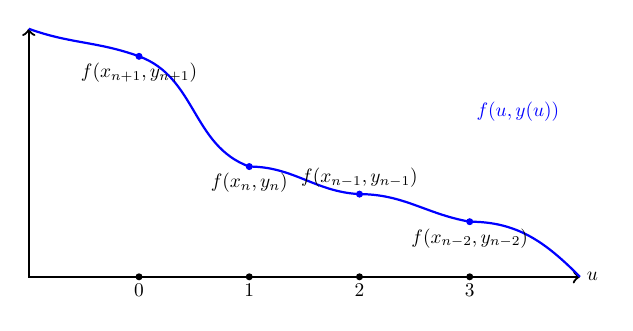
\begin{tikzpicture}[scale=0.7,every node/.style={scale=0.7}]
	% Ejes
	\draw [thick, <->] (0,4.5) -- (0,0) -- (10,0);
	% f(x_n,y_n)
	\begin{scope}[shift={(10,0)},yscale=1,xscale=-1]
		\draw[blue,thick] (0,0) to[out=45,in=180] (2,1);
		\draw[blue,thick] (2,1) to[out=10,in=180] (4,1.5);
		\draw[blue,thick] (4,1.5) to[out=3,in=180] (6,2);
		\draw[blue,thick] (6,2) to[out=20,in=200] (8,4);
		\draw[blue,thick] (8,4) to[out=20,in=200] (10,4.5);
	\end{scope}
	% Labels x_n
	\draw[fill] (2,0) circle [radius=1.5pt];
	\node[below] at (2,0) {$0$};
	\draw[fill] (4,0) circle [radius=1.5pt];
	\node[below] at (4,0) {$1$};
	\draw[fill] (6,0) circle [radius=1.5pt];
	\node[below] at (6,0) {$2$};
	\draw[fill] (8,0) circle [radius=1.5pt];
	\node[below] at (8,0) {$3$};

	% Lables fs
	\draw[blue, fill] (2,4) circle [blue,radius=1.5pt];
	\node[font=\fontsize{10}{144}\selectfont, below] at (2,4) {$f(x_{n+1},y_{n+1})$};
	\draw[blue, fill] (4,2) circle [blue,radius=1.5pt];
	\node[font=\fontsize{10}{144}\selectfont, below] at (4,2) {$f(x_{n},y_{n})$};
	\draw[blue, fill] (6,1.5) circle [blue,radius=1.5pt];
	\node[font=\fontsize{10}{144}\selectfont, above] at (6,1.5) {$f(x_{n-1},y_{n-1})$};
	\draw[blue, fill] (8,1) circle [blue,radius=1.5pt];
	\node[font=\fontsize{10}{144}\selectfont, below] at (8,1) {$f(x_{n-2},y_{n-2})$};

	% General labels
	\node[right] at (10,0) {$u$};
	\node[blue,right] at (8,3) {$f(u,y(u))$};
\end{tikzpicture}